\pagestyle{fancy}
\chapter{Αριθμητική εφαρμογή}
\section{Επίλυση με χρήση απλής αριθμομηχανής}
\subsection{Έλεγχος σε διάτμηση}
\noindent
Με την υπόθεση ίδιου στατικού ύψους και στις δύο διευθύνσεις και χωρίς οπλισμό διάτμησης είναι:
\begin{align*}
s_x &= d + 0.5 c_x + a_x = 0.85m, s'_x = -d - 0.5 c_x + a_x = -0.85m\\[5pt]
s_y &= d + 0.5 c_y + a_y = 0.75m, s'_y = -d - 0.5 c_y + a_y = -0.75m
\end{align*}
\noindent
Είναι $\dfrac{\abs{e_x}}{b_x} = 0.199 > \dfrac{1}{6}$ και $\dfrac{\abs{e_y}}{b_y} = 0.065 \leq \dfrac{1}{6}$ άρα:

\medskip

(Eξ. \ref{eqn:24a}) $\rightarrow V_{Ed,x} = 306.72 KN$

(Eξ. \ref{eqn:24b}) $\rightarrow V'_{Ed,x} = -14.23 KN$

(Eξ. \ref{eqn:25a}) $\rightarrow V_{Ed,y} = 253.34 KN$

(Eξ. \ref{eqn:25b}) $\rightarrow V'_{Ed,y} = 119.75 KN$

\noindent
Για $\rho_{1} = 0.0013$, δηλαδή χρησιμοποιώντας τον κατασκευαστικά ελάχιστο κατά \textlatin{EC2} και στις δύο διευθύνσεις θα είναι:

\medskip

(Eξ. \ref{eqn:27a}) $\rightarrow V_{Rd1,x} = 448.94 KN$

(Eξ. \ref{eqn:27b}) $\rightarrow V_{Rd1,y} = 448.94 KN$

\noindent
Οπότε:
\begin{equation*}
	\left.
	\begin{array}{ll}
		V_{Ed,x,max} & = 306.72 KN \leq V_{Rd1,x} = 448.94 KN\\
		V_{Ed,y,max} & = 253.34 KN \leq V_{Rd1,y} = 448.94 KN
	\end{array}
	\right \} \Rightarrow OK
\end{equation*}

\subsection{Έλεγχος σε διάτρηση}
Κρίσιμη διατομή επιλέγεται αυτή σε απόσταση $a = 0.3m$, η οποία πρόκυπτει στη συνέχεια και από την επίλυση με τη χρήση λογισμικού. Οι τέσσερις πρόβολοι του πεδίλου ορίζουν το γεωμετρικό όριο μέχρι το οποίο αναζητείται η κρίσιμη διατομή.
\begin{align*}
L_{\pi\rho,+x} & = b_x / 2 - c_x / 2 - a_x = 0.85, L_{\pi\rho,-x}  = b_x / 2 - c_x / 2 + a_x = 0.85\\[5pt]
L_{\pi\rho,+y} & = b_x / 2 - c_x / 2 - a_x = 0.95, L_{\pi\rho,-y} = b_x / 2 - c_x / 2 + a_x = 0.95
\end{align*}

\noindent
Από (Eξ. \ref{eqn:28a} - \ref{eqn:28b}), με ${\rho}_1 = max\left(0.26 f_{ctm} / f_{yk}, 0.0013\right) = 0.0013$ είναι:
\begin{equation*}
	\left.
    \begin{array}{ll}
        v_{Rd,c}\left(a\right) & = 1301 KN/{m^2}\\
        v_{Rd,max} & = 3825 KN/{m^2}
    \end{array}
	\right \}\Rightarrow v_{Rd,max} \geq v_{Rd,c}\left(a\right) \Rightarrow OK
\end{equation*}

(Eξ. \ref{eqn:212} - \ref{eqn:213}) $\rightarrow A' = 1.122 m^2$ και $u\left(a\right) = 3.884 m$

(Eξ. \ref{eqn:211}, \ref{eqn:216a}) $\rightarrow V_{Ed,red}\left(a\right) = 851.12 KN$ και $W_f = 119.75 KN$

(Eξ. \ref{eqn:216b} - \ref{eqn:216c}) $\rightarrow I'_x = 0.1001 m^4$ και $I'_y = 0.0756 m^4$

\noindent
Άρα οι μειωμένες ροπές είναι:

(Eξ. \ref{eqn:215a} - \ref{eqn:215b}) $\rightarrow M_{Edx,red}\left(a\right) = 526 KNm$ και $M_{Edy,red}\left(a\right) = 174.16 KNm$

\noindent
Και οι αντίστοιχες εκκεντρότητες:

(Eξ. \ref{eqn:214}) $\rightarrow e_{x,red}\left(a\right) = 0.618 m$ και $e_{y,red}\left(a\right) = 0.204 m$

\noindent
Εφόσον $e_{x,red}\left(a\right) > 0$ και $e_{y,red}\left(a\right) > 0$ από (Eξ. \ref{eqn:221}) θα είναι: $\beta\left(a\right) = 2.153$

\medskip 

\noindent
Άρα τελικά από (Eξ. \ref{eqn:210}) $\rightarrow maxv_{Ed}\left(a\right) = 857.81 KN/m^2$

\medskip

\noindent
Και επίσης: $maxv_{Ed}\left(a\right) \leq v_{Rd,c}\left(a\right)\Rightarrow 857.81 \leq 1301 \Rightarrow OK$ 

\bigskip

\noindent
\textbf{\textcolor{mygreen}{Από τους ελέγχους σε διάτμηση και διάτρηση που διενεργήθηκαν συμπεραίνεται πως το ύψος του πεδίλου επαρκεί.}}

\subsection{Διαστασιολόγηση σε κάμψη}
Κρίσιμες διατομές σε κάμψη είναι οι παράλληλες της περιμέτρου του υποστυλώματος, συνεπώς οι κρίσιμες αποστάσεις που απαιτούνται για την ανάλυση έχουν ως εξής:
\begin{align*}
s_x & = 0.5 c_x + a_x = 0.3m, s'_x =- 0.5 c_x + a_x = -0.3m\\[10pt]
s_y & = 0.5 c_y + a_y = 0.2m, s'_y = - 0.5 c_y + a_y = -0.2m
\end{align*}

\noindent
Είναι $\dfrac{\abs{e_x}}{b_x} = 0.199 > \dfrac{1}{6}$ και $\dfrac{\abs{e_y}}{b_y} = 0.065 \leq \dfrac{1}{6}$ άρα:

\medskip

(Eξ. \ref{eqn:223a}) $\rightarrow M_{Ed,x} = 340.42 KNm$

(Eξ. \ref{eqn:223b}) $\rightarrow M'_{Ed,x} = 3.56 KNm$

(Eξ. \ref{eqn:224a}) $\rightarrow M_{Ed,y} = 276.97 KNm$

(Eξ. \ref{eqn:224b}) $\rightarrow M'_{Ed,y} = 144.18 KNm$

\noindent
Από τους παραπάνω υπολογισμούς προκύπτει $M_{Ed,x,max} = 340.42 KNm$ και $M_{Ed,y,max} = 276.97 KNm$.

\begin{itemize}
	\item Διεύθυνση $x$:\\
	Για τη μέγιστη ροπή, ανά μονάδα πλάτους του πεδίλου θα είναι $340.42 / 2.3 = 148 KNm/m$. Οι κρίσιμες σε κάμψη διατομές απέχουν από το άκρο του πεδίλου $l = 1.15 - 0.3 = 0.85 m \leq 2d = 1.1m$. Άρα εμφανίζεται κοντός πρόβολος, συνεπώς λαμβάνεται προσεγγιστικά $z = 0.85d$ και είναι $A_s = \dfrac{M_{sd}}{0.85\cdot d \cdot f_{yd}}$.
	\begin{itemize}
		\item Απαιτούμενος οπλισμός: $A_s = \dfrac{148}{0.85\cdot0.55\cdot434.78} = 728{mm}^2 / m$
		\item Κατασκευαστικά ελάχιστος οπλισμός: $A_{s,min} = 0.0013\cdot1000\cdot550 = 715{mm}^2 / m$
		\item Τοποθετούνται $\Phi 14/200 = 770{mm}^2 / m$
	\end{itemize}
	\item Διεύθυνση $y$:\\
	Για τη μέγιστη ροπή, ανά μονάδα πλάτους του πεδίλου θα είναι $276.97 / 2.3 = 120.4 KNm/m$. Οι κρίσιμες σε κάμψη διατομές απέχουν από το άκρο του πεδίλου $l = 1.15 - 0.2 = 0.95 m \leq 2d = 1.1m$. Άρα εμφανίζεται κοντός πρόβολος, συνεπώς λαμβάνεται προσεγγιστικά $z = 0.85 d$ και είναι $A_s = \dfrac{M_{sd}}{0.85 \cdot d \cdot f_{yd}}$.
	\begin{itemize}
		\item Απαιτούμενος οπλισμός: $A_s = \dfrac{120.4}{0.85\cdot0.55\cdot434.78} = 592{mm}^2 / m$
		\item Κατασκευαστικά ελάχιστος οπλισμός: $A_{s,min} = 0.0013\cdot1000\cdot550 = 715{mm}^2 / m$
		\item Τοποθετούνται $\Phi 14/200 = 770{mm}^2 / m$
	\end{itemize}
\end{itemize}

\section{Επίλυση με χρήση λογισμικού}
Στο παρόν μέρος παρουσιάζονται τα αποτελέσματα επίλυσης του τμήματος της προηγούμενης αριθμητικής εφαρμογής που αφορά τον έλεγχο σε διάτρηση. Τα παρακάτω αποτελέσματα (Πίν. \ref{tab:results}) παρήχθησαν με λογισμικό που αναπτύχθηκε σε γλώσσα \textlatin{C++} (βλ. Παράρτημα) και υπολογίζει τη μεταβολή  του λόγου αντοχής προς καταπόνηση για τις διάφορες τιμές του $a$ (Σχ. \ref{fig:chart}). Σημειώνεται πως οι δύο μέθοδοι συγκλίνουν σε ικανοποιητικό βαθμό, αλλά γενικώς η χρήση Η/Υ συνίσταται για μεγαλύτερη ακρίβεια αποτελεσμάτων και σαφή μείωση του υπολογιστικού φόρτου. Βέβαια, απαραίτητη προϋπόθεση για το τελευταίο, αποτελεί η πλήρης κατανόηση του εκάστοτε προβλήματος και των σχέσεων που το περιγράφουν.

\begin{figure}[H]
  \centering
  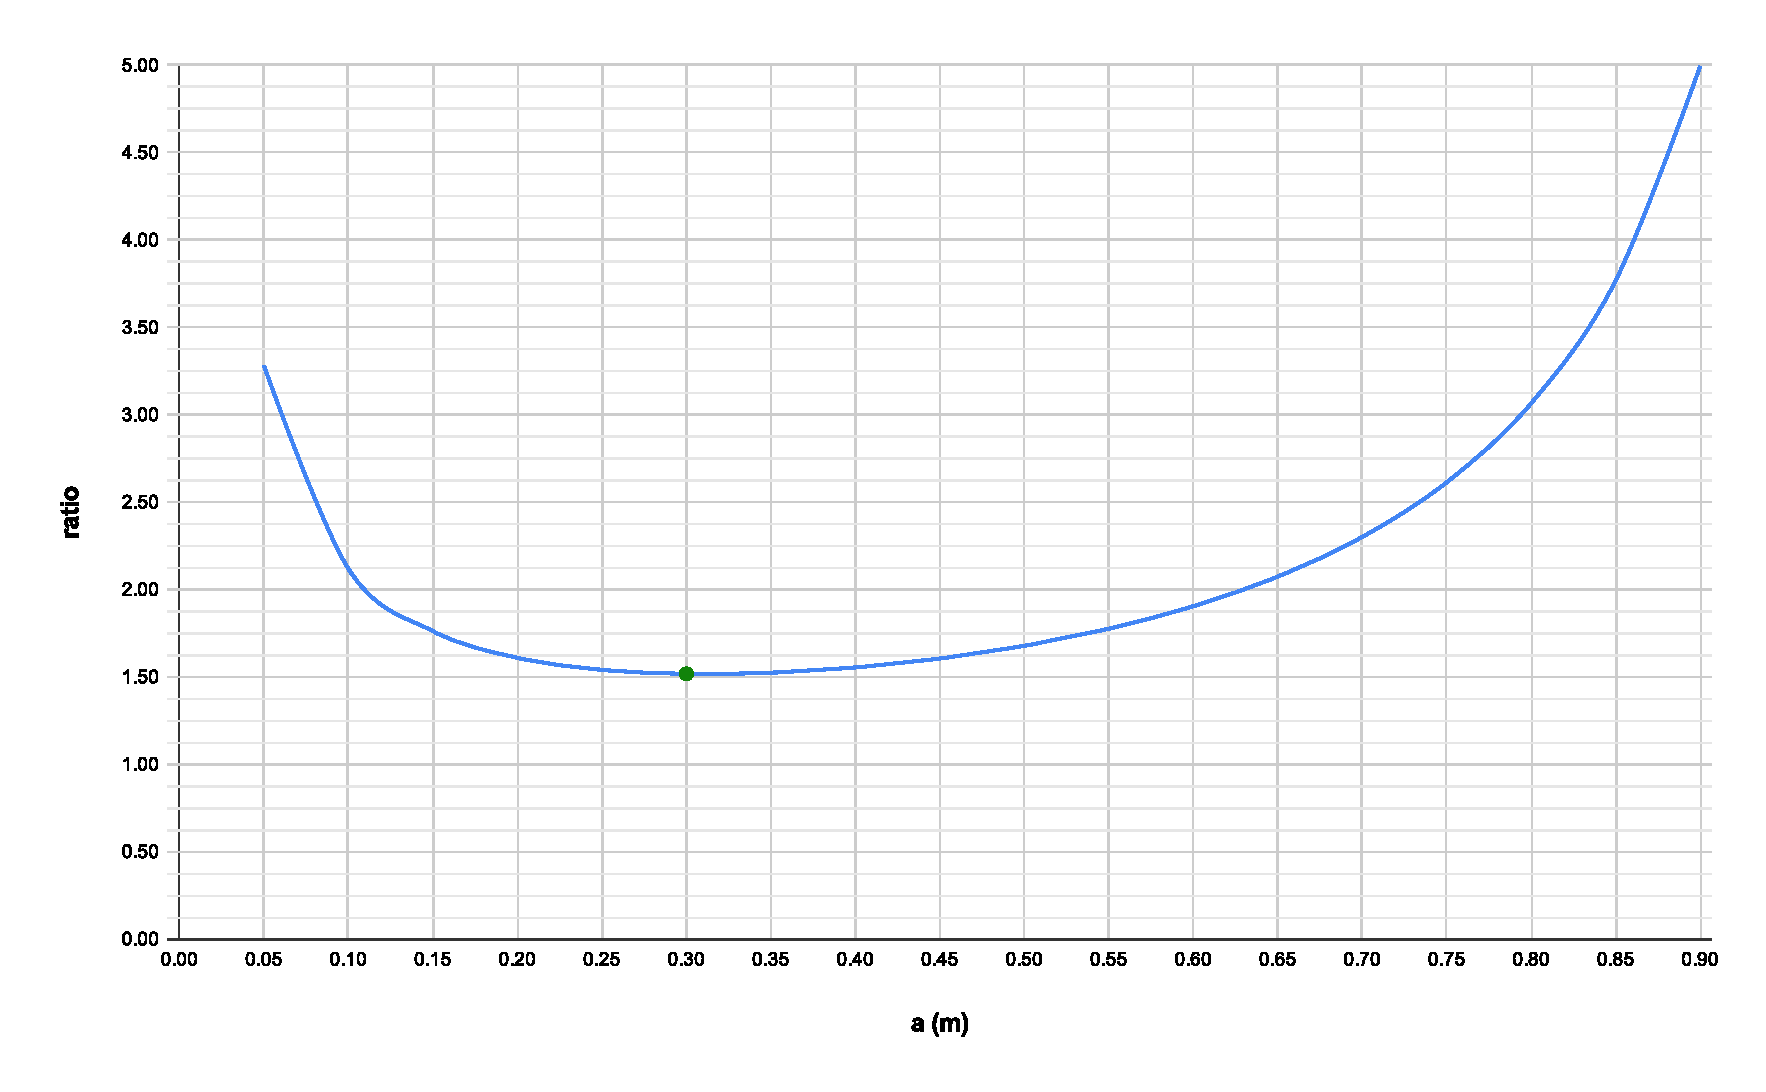
\includegraphics[width=\textwidth,keepaspectratio]{chart}
  \caption{Μεταβολή του λόγου αντοχής προς καταπόνηση για τις διάφορες τιμές του \textlatin{a}}
  \label{fig:chart}
\end{figure}

\begin{landscape}
\begin{table}[H]
\centering\setlength{\arrayrulewidth}{0.3mm}
\begin{tabular}{| c | c | c | c | c | c | c | c | c | c | c | c | c | c | c |}
\hline
$\mathbf{a}$ & $\mathbf{inside}$ & $\mathbf{u}$ & $\mathbf{A'}$ & $\mathbf{V_{Ed,red}}$ & $\mathbf{I'_x}$ & $\mathbf{I'_y}$ & $\mathbf{M_{Edx,red}}$ & $\mathbf{M_{Edy,red}}$ & $\mathbf{e_{x,red}}$ & $\mathbf{e_{y,red}}$ & $\mathbf{\beta}$ & $\mathbf{v_{Rd,c}}$ & $\mathbf{maxv_{Ed}}$ & $\mathbf{v_{Rd,c}/maxv_{Ed}}$ \\
$(m)$ & $-$ & $(m)$ & $(m^2)$ & $(KN)$ & $(m^4)$ & $(m^4)$ & $(KNm)$ & $(KNm)$ & $(m)$ & $(m)$ & $-$ & $(KN/m^2)$ & $(KN/m^2)$ & $-$ \\
\hline
$0.00$ & $true$ & $2.000$ & $0.240$ & $1031.24$ & $0.0072$ & $0.0032$ & $548.30$ & $179.75$ & $0.531$ & $0.174$ & $3.449$ & $inf$ & $3233.49$ & $inf$ \\
\hline
$0.05$ & $true$ & $2.314$ & $0.347$ & $1009.21$ & $0.0139$ & $0.0071$ & $546.71$ & $179.45$ & $0.541$ & $0.177$ & $3.003$ & $7813.94$ & $2381.18$ & $3.28153$ \\
\hline
$0.10$ & $true$ & $2.628$ & $0.471$ & $983.98$ & $0.0235$ & $0.0132$ & $544.44$ & $178.98$ & $0.553$ & $0.181$ & $2.709$ & $3906.97$ & $1844.39$ & $2.11829$ \\
\hline
$0.15$ & $true$ & $2.942$ & $0.610$ & $955.54$ & $0.0364$ & $0.0219$ & $541.40$ & $178.30$ & $0.566$ & $0.186$ & $2.503$ & $2604.64$ & $1478.44$ & $1.76174$ \\
\hline
$0.20$ & $true$ & $3.256$ & $0.765$ & $923.89$ & $0.0531$ & $0.0340$ & $537.47$ & $177.37$ & $0.581$ & $0.191$ & $2.353$ & $1953.48$ & $1214.11$ & $1.60898$ \\
\hline
$0.25$ & $true$ & $3.570$ & $0.936$ & $889.04$ & $0.0741$ & $0.0500$ & $532.52$ & $176.13$ & $0.598$ & $0.198$ & $2.241$ & $1562.78$ & $1014.49$ & $1.54047$ \\
\hline
$\color{myred}0.30$ & $\color{myred}true$ & $\color{myred}3.884$ & $\color{myred}1.122$ & $\color{myred}850.97$ & $\color{myred}0.1002$ & $\color{myred}0.0708$ & $\color{myred}526.36$ & $\color{myred}174.52$ & $\color{myred}0.618$ & $\color{myred}0.205$ & $\color{myred}2.155$ & $\color{myred}1302.32$ & $\color{myred}858.29$ & $\color{myred}1.51734$ \\
\hline
$0.35$ & $true$ & $4.199$ & $1.324$ & $809.70$ & $0.1322$ & $0.0974$ & $518.80$ & $172.47$ & $0.640$ & $0.213$ & $2.089$ & $1116.27$ & $732.45$ & $1.52402$ \\
\hline
$0.40$ & $true$ & $4.513$ & $1.542$ & $765.23$ & $0.1712$ & $0.1308$ & $509.62$ & $169.89$ & $0.665$ & $0.222$ & $2.038$ & $976.74$ & $628.55$ & $1.55395$ \\
\hline
$0.45$ & $true$ & $4.827$ & $1.776$ & $717.54$ & $0.2181$ & $0.1723$ & $498.54$ & $166.70$ & $0.694$ & $0.232$ & $2.001$ & $868.21$ & $540.93$ & $1.60502$ \\
\hline
$0.50$ & $true$ & $5.141$ & $2.025$ & $666.65$ & $0.2743$ & $0.2230$ & $485.30$ & $162.78$ & $0.727$ & $0.244$ & $1.975$ & $781.39$ & $465.69$ & $1.67790$ \\
\hline
$0.55$ & $true$ & $5.455$ & $2.290$ & $612.55$ & $0.3409$ & $0.2845$ & $469.58$ & $158.04$ & $0.766$ & $0.258$ & $1.959$ & $710.35$ & $400.03$ & $1.77574$ \\
\hline
$0.60$ & $true$ & $5.769$ & $2.570$ & $555.24$ & $0.4195$ & $0.3582$ & $451.04$ & $152.34$ & $0.812$ & $0.274$ & $1.954$ & $651.16$ & $341.91$ & $1.90447$ \\
\hline
$0.65$ & $true$ & $6.084$ & $2.867$ & $494.72$ & $0.5116$ & $0.4458$ & $429.31$ & $145.58$ & $0.867$ & $0.294$ & $1.960$ & $601.07$ & $289.80$ & $2.07405$ \\
\hline
$0.70$ & $true$ & $6.398$ & $3.179$ & $431.00$ & $0.6189$ & $0.5492$ & $404.01$ & $137.60$ & $0.937$ & $0.319$ & $1.980$ & $558.13$ & $242.55$ & $2.30104$ \\
\hline
$0.75$ & $true$ & $6.712$ & $3.507$ & $364.06$ & $0.7432$ & $0.6701$ & $374.70$ & $128.27$ & $1.029$ & $0.352$ & $2.020$ & $520.92$ & $199.27$ & $2.61410$ \\
\hline
$0.80$ & $true$ & $7.026$ & $3.850$ & $293.93$ & $0.8863$ & $0.8106$ & $340.94$ & $117.42$ & $1.159$ & $0.399$ & $2.093$ & $488.37$ & $159.25$ & $3.06652$ \\
\hline
$0.85$ & $false$ & $7.340$ & $4.209$ & $220.58$ & $1.0504$ & $0.9728$ & $302.25$ & $104.90$ & $1.370$ & $0.475$ & $2.232$ & $459.64$ & $121.94$ & $3.76912$ \\
\hline
$0.90$ & $false$ & $7.654$ & $4.584$ & $144.02$ & $1.2375$ & $1.1590$ & $258.13$ & $90.53$ & $1.792$ & $0.628$ & $2.540$ & $434.10$ & $86.90$ & $4.99535$ \\
\hline
\end{tabular}
\caption{Αποτελέσματα (\textlatin{output}) του προγράμματος και κρίσιμη διατομή}
\label{tab:results}
\end{table}
\end{landscape}